\documentclass[12pt,a4paper]{article}

\usepackage[utf8]{inputenc}
\usepackage[T2A]{fontenc}
\usepackage[english,russian]{babel}
\usepackage{array}
\usepackage{booktabs}
\usepackage{geometry}
\usepackage{graphicx}
\usepackage{hyperref}
\usepackage{longtable}
\geometry{margin=25mm}
\hypersetup{unicode=true,colorlinks=true,urlcolor=blue,linkcolor=black}
\newcommand{\code}[1]{\texttt{\detokenize{#1}}}

\begin{document}

\begin{titlepage}
\begin{center}
{\large Московский авиационный институт\\
(национальный исследовательский университет)}

\vfill
Лабораторная работа по курсу «Информационный поиск»

\vspace{12mm}
{\Large \textbf{Лабораторная работа №1}}\\
{\large \textbf{Добыча корпуса документов}}

\vfill
\begin{flushright}
Студент: К.\,А. Арусланов\\
Группа: \underline{\hspace{45mm}}\\
Преподаватель: А.\,А. Кухтичев\\
Дата: \underline{\hspace{45mm}}\\
Оценка: \underline{\hspace{45mm}}
\end{flushright}

\vfill
Москва, 2026
\end{center}
\end{titlepage}

\tableofcontents
\newpage

\section{Постановка задачи}

Необходимо скачать примеры документов будущего корпуса, изучить их разметку
и метаданные, выделить основной текст, найти внешние средства поиска и
посчитать характеристики выборки. Темой корпуса выбраны русскоязычные
редакционные публикации о видеоиграх и игровой индустрии: новости, статьи,
обзоры, превью и аналитика.

\section{Источники и метод}

Кандидатами являются PlayGround.ru, StopGame.ru, IXBT.games и Игромания.
В окончательном корпусе будет не менее двух независимых источников. В
\code{urls.txt} подготовлено 15 репрезентативных страниц: 3 PlayGround, 5
StopGame, 4 IXBT.games и 3 Игромании. Массовый обход на этапе лабораторной
работы не выполняется.

Сбор запускается командой:

\begin{verbatim}
python main.py collect urls.txt --delay 2
\end{verbatim}

Перед запросом программа получает и сохраняет актуальный \code{robots.txt},
проверяет URL для собственного User-Agent и не запрашивает запрещённые пути.
Ответ классифицируется как документ, редирект, 404, 429, 5xx,
anti-bot/challenge или запрет robots.txt. CAPTCHA и WAF не обходятся.

Сырой HTML хранится в \code{data/raw/<source>/}, JSON с результатом
разбора --- в \code{data/parsed/<source>/}. Путь к исходному HTML хранится
в JSON, поэтому после изменения парсера возможен повторный разбор без сети:
\code{python main.py reparse}.

\section{Единая модель документа}

Все парсеры возвращают источник, URL, заголовок, автора, дату публикации,
категорию, теги, связанные игры, основной текст и исходные метаданные. Также
записываются HTTP-статус, размеры сырого и выделенного текста, SHA-256
нормализованного текста и ошибка разбора. Неизвестные метаданные не
выдумываются. Удаляются только tracking-параметры URL, а содержательные
параметры сохраняются.

\section{Разметка и выделение текста}

Правила ниже проверены на 15 сохранённых HTML: по 3 страницам PlayGround и
Игромании, 4 IXBT.games и 5 StopGame. В каждом случае найден ровно один
контейнер основного текста и выделено более 100 слов.

\begin{center}
\begin{tabular}{p{0.19\linewidth}p{0.34\linewidth}p{0.34\linewidth}}
\toprule
Источник & Основной текст & Категория и таксономия \\
\midrule
PlayGround & \code{div.article-content} & URL: \code{news} $\rightarrow$ news,
\code{opinion} $\rightarrow$ review; JSON-LD \code{about.name} $\rightarrow$
games \\
StopGame & \code{article#material_content} & \code{newsdata} $\rightarrow$
news; \code{show} с «обзор» $\rightarrow$ review; теги и игры извлекаются из
ссылок \\
IXBT.games & \code{div[id^="publication-"].prose} & JSON-LD
\code{articleSection}: новости, статьи, обзоры $\rightarrow$ news, article,
review \\
Игромания & \code{div[class*="material-content_"]} & JSON-LD \code{@type}:
\code{NewsArticle}, \code{Article}, \code{Review}; блок тегов $\rightarrow$
tags \\
\bottomrule
\end{tabular}
\end{center}

Для всех сайтов заголовок и служебные поля берутся из \code{h1} и JSON-LD
\code{headline}, \code{author}, \code{datePublished}. У PlayGround внешний
\code{article} включает комментарии и рекомендации. В IXBT.games числовая
часть ID динамическая, а у Игромании динамичен суффикс CSS Modules, поэтому
используются устойчивые фрагменты селекторов. Теги Игромании дублируются в
desktop/mobile-блоках и дедуплицируются. В StopGame блоки \code{_read-more}
ссылаются на другие материалы и удаляются до извлечения. На проверенных
страницах IXBT.games нет надёжных тегов или имён игр, поэтому эти поля не
заполняются догадками.

\section{Статистика проверочной выборки}

Локально сохранены и разобраны все 15 страниц из \code{urls.txt}. Повторный
разбор выполняется без обращения к сети:

\begin{verbatim}
python main.py reparse
python main.py stats
\end{verbatim}

\begin{center}
\begin{tabular}{lr}
\toprule
Показатель & Значение \\
\midrule
Количество документов & 15 \\
Успешно распарсено / ошибок & 15 / 0 \\
Размер сырого HTML & 3\,902\,865 байт \\
Размер выделенного текста & 257\,344 байта \\
Средний raw / text & 260\,191 / 17\,156 байт \\
Медиана текста & 11\,588 байт \\
Минимум / максимум текста & 1\,792 / 59\,797 байт \\
Слов всего & 20\,592 \\
Среднее / медиана слов & 1\,372.8 / 943 \\
Точных дубликатов & 0 \\
Коэффициент извлечения & 6.5937\% \\
\bottomrule
\end{tabular}
\end{center}

Распределение документов: PlayGround --- 3, StopGame --- 5, IXBT.games --- 4,
Игромания --- 3. Это техническая выборка для проверки разметки; её нельзя
экстраполировать на миллион документов или считать финальным корпусом.

\begin{center}
\begin{tabular}{lrrrrr}
\toprule
Источник & Док. & Raw, байт & Текст, байт & Средний текст & Слов \\
\midrule
PlayGround & 3 & 638\,220 & 34\,087 & 11\,362 & 2\,680 \\
StopGame & 5 & 1\,250\,938 & 103\,672 & 20\,734 & 8\,524 \\
IXBT.games & 4 & 1\,238\,733 & 59\,505 & 14\,876 & 4\,671 \\
Игромания & 3 & 774\,974 & 60\,080 & 20\,027 & 4\,717 \\
\bottomrule
\end{tabular}
\end{center}

\section{Существующий поиск}

Корпус доступен во встроенных поисках сайтов и во внешних поисковиках с
ограничением \code{site:}. Проверка проведена 19 сентября 2026 года. Для
каждого кейса известен документ, который должен быть найден, поэтому
недостатки выдачи проверяются сравнением результатов с сохранёнными HTML и
выделенным текстом.

\begin{longtable}{p{0.26\linewidth}p{0.34\linewidth}p{0.27\linewidth}}
\toprule
Запрос и ожидаемый документ & Наблюдение & Недостаток \\
\midrule
\endfirsthead
\toprule
Запрос и ожидаемый документ & Наблюдение & Недостаток \\
\midrule
\endhead
«джо кросс»: новости о Джозефе Кроссе на StopGame и Игромании &
Внутренний поиск StopGame выдаёт «кроссовер» и «кросс-плей». Яндекс с
\code{site:stopgame.ru} не находит релевантную новость, а для Игромании
показывает один документ. Google показывает релевантные публикации обоих
сайтов в первых позициях. & Полнота зависит от поисковой системы; внутренний
поиск StopGame плохо обрабатывает вариант имени «Джо/Джозеф Кросс». \\
«приземлённый подход Insomniac» из статьи IXBT.games о Marvel's
Wolverine & Внутренний поиск IXBT.games сообщает «Ничего не найдено», хотя
фраза содержится в статье. Яндекс с \code{site:ixbt.games} находит её первой.
& Внутренний поиск не гарантирует поиск по полному тексту. \\
«я играю роль поп-звезды, которая убила себя на сцене» из блога
StopGame «Музыка Ночного Города» & Внутренний поиск StopGame возвращает
несвязанные блоги; Яндекс выводит нужный блог первым. & Даже точная фраза не
даёт ожидаемого результата; используемые токенизация и ранжирование
непрозрачны. \\
«леман» на StopGame & Первый результат --- «Косплемания: Chummomo...».
Искомая последовательность присутствует лишь внутри слова «Косплемания», а
не как сущность «Ле-Ман». & Сопоставление подстроки без границ слова даёт
тематически нерелевантный результат. \\
Отбор по типу публикации & В просмотренных интерфейсах IXBT.games и Игромании
нет группировки на новости, статьи и блоги; в StopGame есть вкладки типов и
сортировка. & Часть внешних и встроенных поисков не использует поля корпуса
\code{category}, \code{tags}, \code{games}; собственной системе нужны
фильтры и зонный поиск. \\
\bottomrule
\end{longtable}

\begin{figure}[htbp]
\centering
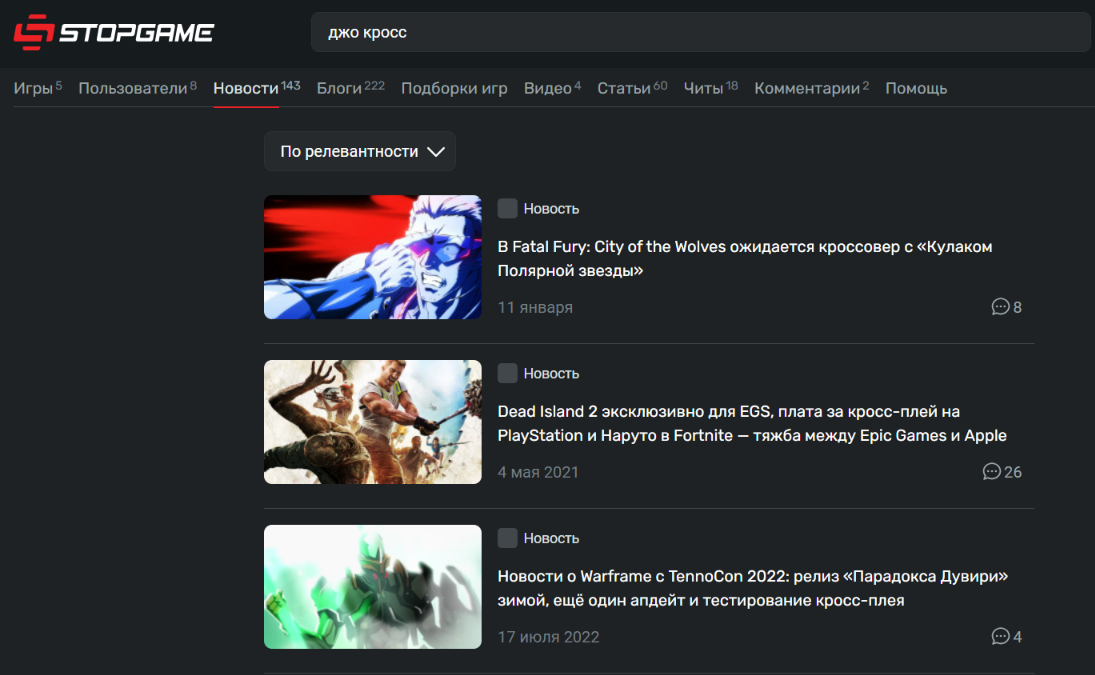
\includegraphics[width=0.47\linewidth]{img/cross_sg.png}\hfill
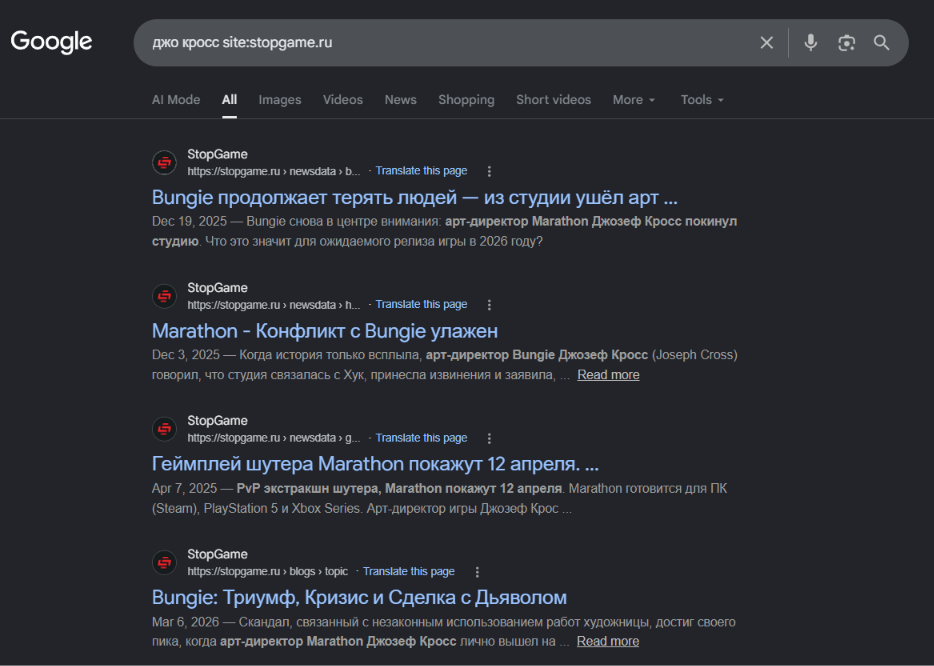
\includegraphics[width=0.47\linewidth]{img/cross_ggl_sg.png}
\caption{Запрос «джо кросс»: нерелевантные результаты встроенного поиска
StopGame (слева) и релевантные результаты Google с ограничением на сайт
(справа).}
\end{figure}

\begin{figure}[htbp]
\centering
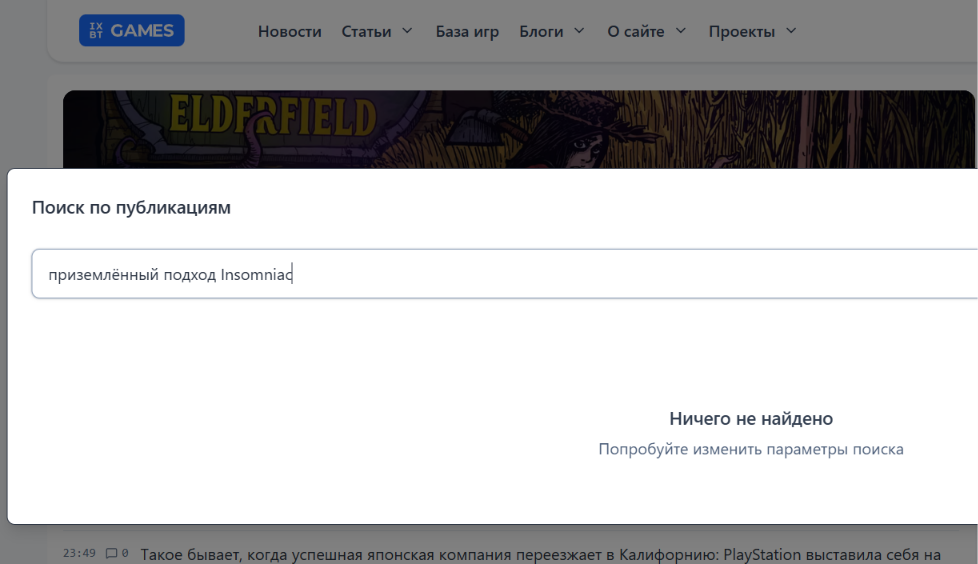
\includegraphics[width=0.47\linewidth]{img/insomniac_ixbt.png}\hfill
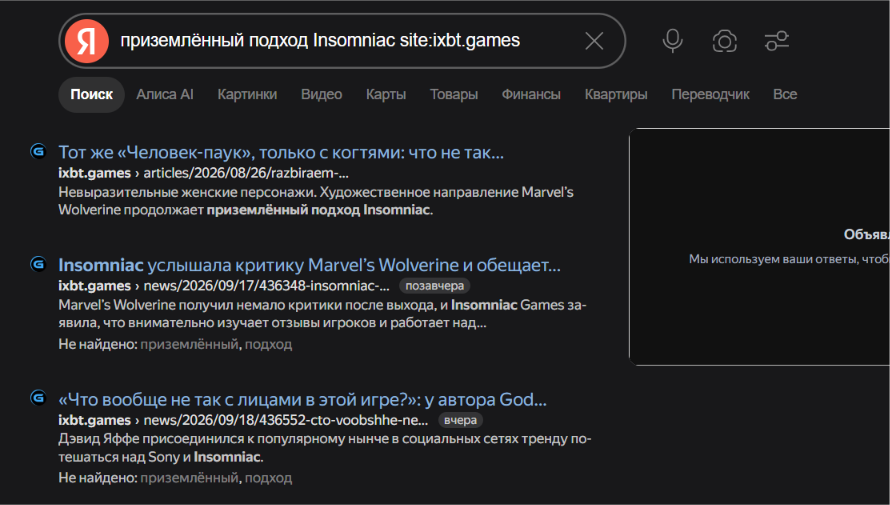
\includegraphics[width=0.47\linewidth]{img/insomniac_ya.png}
\caption{Точная фраза из статьи IXBT.games не находится внутренним поиском
(слева), но находится Яндексом с \code{site:ixbt.games} (справа).}
\end{figure}

\begin{figure}[htbp]
\centering
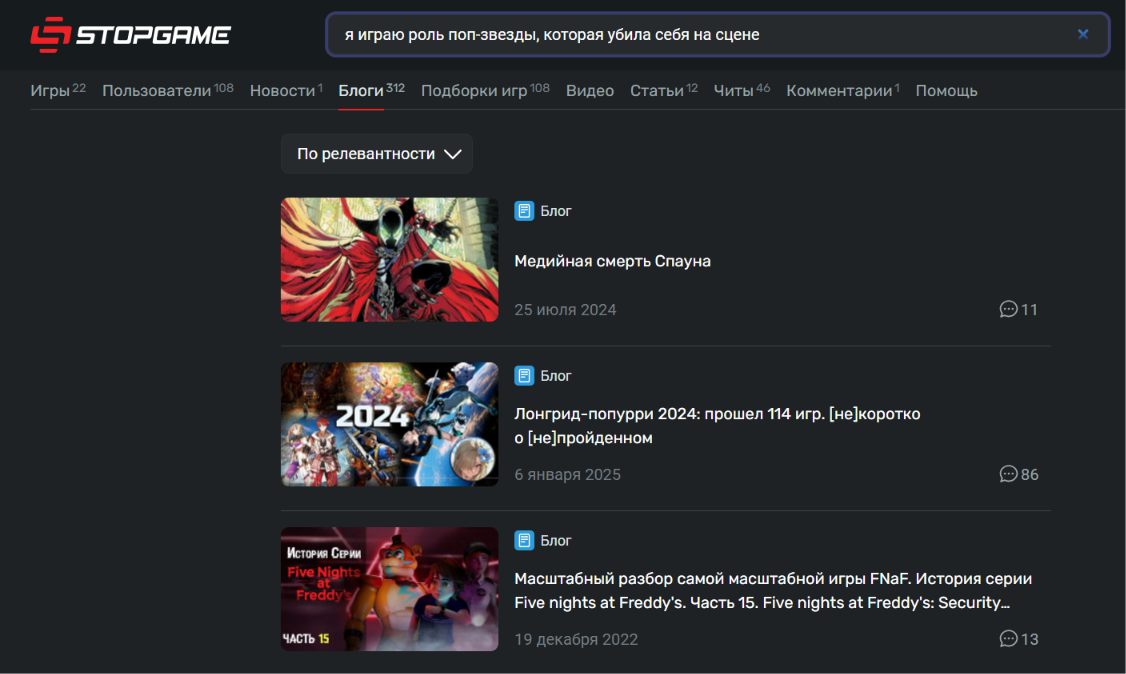
\includegraphics[width=0.47\linewidth]{img/pop_sg.png}\hfill
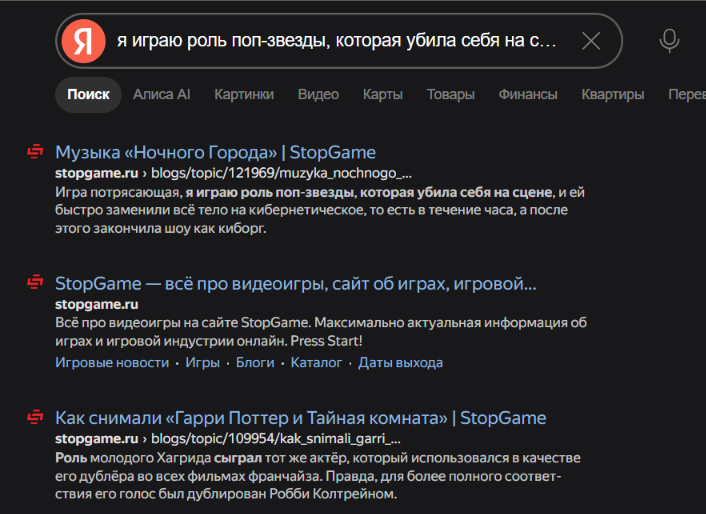
\includegraphics[width=0.47\linewidth]{img/pop_ya_sg.png}
\caption{Поиск точной цитаты из блога StopGame: встроенный поиск возвращает
другие блоги (слева), Яндекс --- нужный документ первым (справа).}
\end{figure}

\begin{figure}[htbp]
\centering
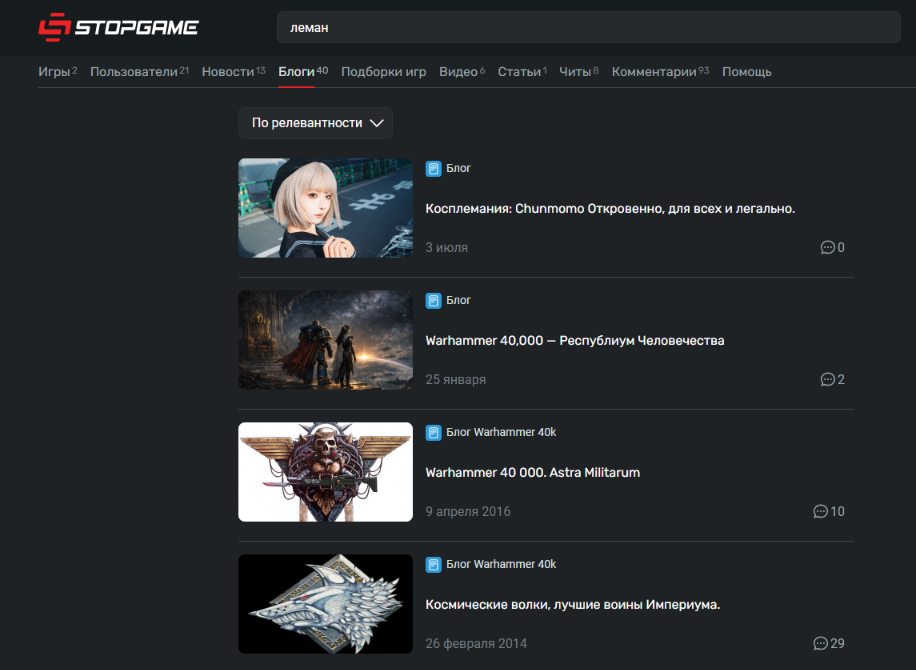
\includegraphics[width=0.47\linewidth]{img/leman_sg.png}\hfill
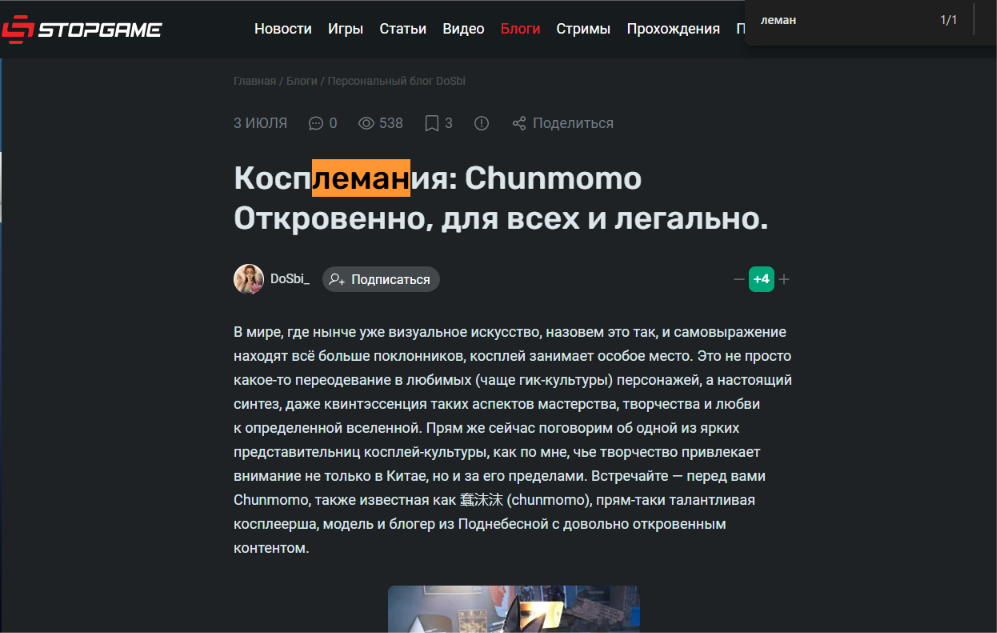
\includegraphics[width=0.47\linewidth]{img/leman_sg_2.png}
\caption{Ложное совпадение по подстроке «леман»: первый результат (слева) и
контекст совпадения внутри слова «Косплемания» (справа).}
\end{figure}

Таким образом, существующие поиски достаточны как внешний ориентир, но не как
замена собственного индекса: у них нет контролируемой полноты, единой
нормализации русских слов и доступа к выделенному основному тексту или
метаданным корпуса.

\section{Тестирование}

Запуск тестов:

\begin{verbatim}
python -m unittest discover -s tests -v
\end{verbatim}

Выполненный прогон содержит пять успешных тестов: проверку селектора StopGame
и исключения связанных блоков, статистику fixtures без дубликатов,
канонизацию URL, а также повторный разбор всех 15 HTML с подтверждёнными
селекторами и проверку таксономии. Далее полезно добавить fixtures для 404,
429, robots.txt и challenge-страницы.

\section{Вывод}

Подготовлена воспроизводимая основа игрового корпуса: общий формат документа,
сохранение raw HTML, диагностика ответов, повторный разбор без сети,
статистика и подтверждённые парсеры для четырёх независимых источников.
Диагностическая часть ЛР~1 выполнена. Перед целью более одного миллиона
документов требуется отдельно посчитать допустимые URL по sitemap/RSS и
разбить обход на контролируемые партии.

\end{document}
